\section{Experimental Analysis}
\label{sec:experimentdesign}

We performed a set of simulations to evaluate the performance of the heuristic algorithms and leverage the white space band influence on mesh network. 
The experiment set up is introduced in \ref{subsec:design} with the topology, metric calculation.
A set of result is shown in ~\ref{subsec:analysis} and analysis is presented with the throughput achieve through gateways.
CCA simplily pick two nodes have common channel to build links which also could be used in multiband scenario.
In BFS-CA, we adopt the ranking standard as single link interference numbers, utilization of channels to fit multiband scenario.


\subsection{Experiment Design}
\label{subsec:design}
% Simulation Setup
We consider static wireless mesh networks with n nodes located in a regular grid with distance of $300m$. 
Today's white space equipment use frequency shift moving signal from white space to WiFi frequency for processing ~\cite{Ubnt}.
We set the RSSI threshold as $-160dBm$ for WiFi and $-154dBm$ for White Space Band adjusting the system loss on the radios ~\cite{cui2013leveraging}.
Then calculate the communication range and double as the interference range~\cite{raniwala2005architecture}. The gateways are randomly selected $\frac{1}{6}$ from the nodes in the network.
We set up to use WiFi band $2.4 GHz$, $5 GHz$ and white space band $450 MHz$, $800 MHz$ to generate the network topology.

ISP such as AT\&T, T-mobile will charge fee according to the traffic arrived at Internet through wireless network. 
They are interested in getting the more throughput achieve gateways, which is the throughput arrived at the gateways from all the mesh nodes. 

Stefano brings the throughput achieve gateways in the network without considering the interference as maximum throughput to evaluate the channel assignment ~\cite{avallone2008channel}. 
However, without considering the interference, the traffic flow in the network is not scheduled.

The throughput achieve gateways binds with multiple factors, such as gateway placement, routing and also channel assignment.
To find the best gateway placement, routing associate with channel assignment is out of our scope. 
In a mesh network, the bottleneck of the network are the links around the gateway nodes ~\cite{robinson2010deploying}. 
And any traffic transmitted to a wired gateway node is treated equally as throughput achieve gateways. 
So a methodology to get a scheduler maximum throughput is to serve the nodes close to the gateway nodes first.
We first serve the nodes have 1 hop path to the gateway nodes, with the same hop count in the path, choose the path has the least interference on the network and serve the demand as more as possible. 
Then we satisfy the demand of multiple hop layer nodes and so on, till there is no demand could be satisfied through any path.
The calculation process is kind of routing protocol which help us to reach a scrollable maximum throughput achieve gateways of the network. 
We would not claim it is the best way, for evaluation we keep the same calculation process for all comparable setting.
% Validation
We relax our ILP model to keep the link capacity constraints, given the demand of the mesh nodes as parameter to get an maximum throughput achieve gateways as shown in ~\ref{fig:varysize}. The up-bound is assuming the mesh node could be connect to all the gateways if there is a path. But we limit a mesh node only connect to one gateway in the network, this bring the difference from the up-bound to our calculation.


% FIXME may need a validation of max calculation

\subsection{Analysis}
\label{subsec:analysis}


% ILP bound

Most of the time clients of wireless network have different traffic demand. The uplink and dwon link traffic are equally occupy the channel capacity.
   Then we randomly assign demand of mesh nodes with a max offer load,
   calculate the scalable maximum throughput, then repeat the process 20 times.
   In the ILP bound, we keep the connectivity constraints in ~\ref{subsec:linearopt}. To simiplify the process, we remove the uplink constraints and keep download demand constraints only. 
   Modify the constraint ~\ref{opt:8} as 
   $\sum_{l \in B} \sum_{j \in V} \sum_{k \in V} dy^k_{j,i,l} \lq \sum_{l \in B} \sum_{j \in V} \sum_{k \in V} dy^k_{i,j,k}+D_{di}, i \neq l$. 
   Maximum $\sum_{i\in Gateway} (D_{di}+\sum_{l\in B,j\in V, k \in V}dy^l_{i,j,k}$.
The output is the average maximum throughput achieve gateways for the max offer load per mesh node.
To evaluate the performance in different size of network, we fix the max offer load of each node as $4MB/s$ and vary the number of nodes in the regular grid network. The performance of the algorithms are shown in ~\ref{fig:varysize}. 
   \begin{figure}
   %\vspace{-0.0in}
   \centering
   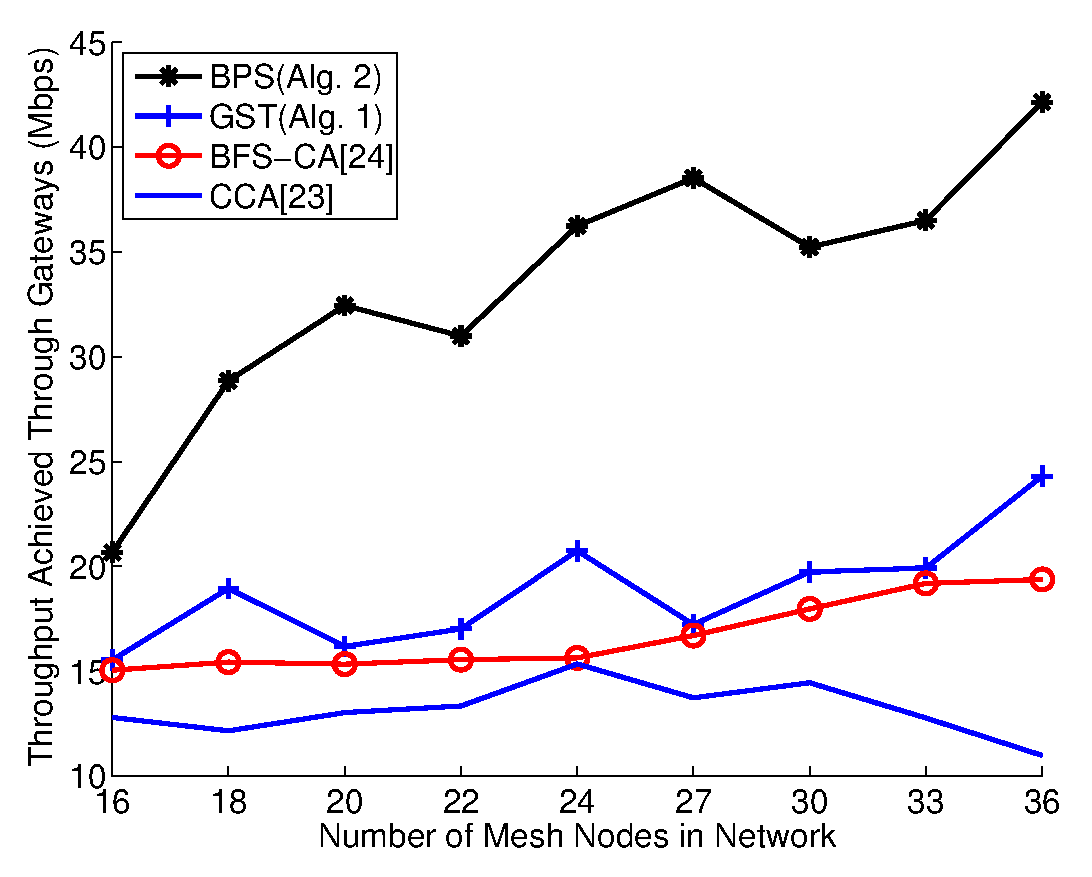
\includegraphics[width=74mm]{figures/varysize}
   \vspace{-0.1in}
   \caption{Uniform offered load per mesh node of 4 Mbps.}                                                                 
   \label{fig:varysize}
   %\vspace{-0.0in}
   \end{figure}

The ILP Bound could have multiple gateway connection but other assignment would have only one gateway connection. And ILP optimize both channel assignment and routing simultaneously.  
As the number of mesh node increase, CCA lose the ability to handle large size of network. 
The dips of the curves are resulting from the random demand evaluation setup.
We randomly deploy the gateways and offer load of each mesh node, brings the decrease in achieving throughput when the number of mesh node increase. 


   The performance of the two heuristic algorithms and ~\emph{CCA} ~\cite{draves2004routing}, ~\emph{BFSCA}  ~\cite{ramachandran2006interference} in a 30-node regular grid topology with 6MB link capacity in each channel are shown in figure ~\ref{fig:maxtpt}.

   \begin{figure}
   %\vspace{-0.0in}
   \centering
   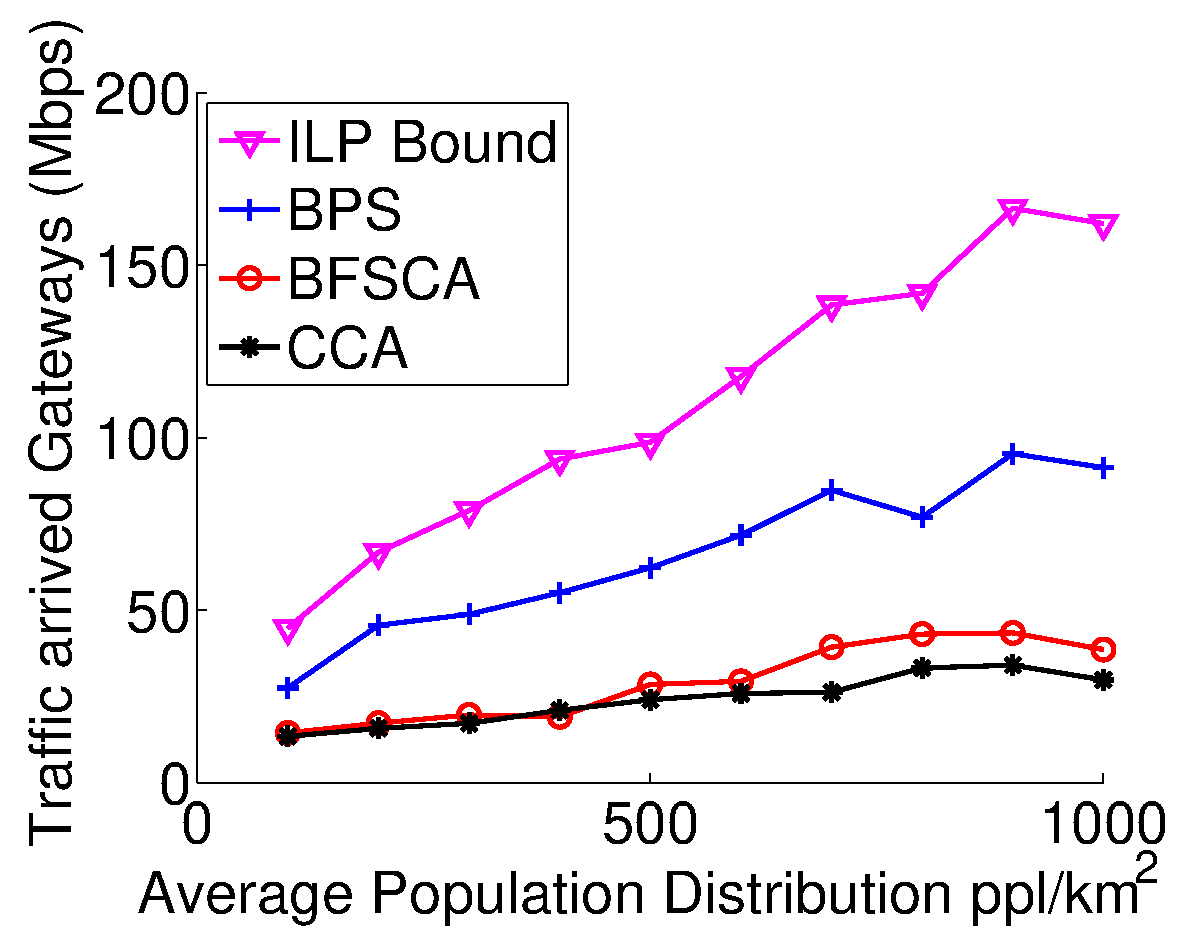
\includegraphics[width=74mm]{figures/maxtpt}
   \vspace{-0.1in}
   \caption{Varying maximum offered load for a 30-node regular-grid mesh topology.}                                                                               
   \label{fig:maxtpt}
   %\vspace{-0.0in}
   \end{figure}
 
   BPS performs better than the other 3 algorithms since during the channel assignment process, it is already optimize the paths from further nodes to gateways make it possible to ship data from these nodes. But as the max offer load increase, all the channel assignment suffer the bottle neck of link capacity.
   GST is trying to optimizing the output of BFS-CA, reducing the hop counts and interference of each hop layer. However, since the 1 hop layer has been assigned throughput BFS-CA which is the bottle neck for the capacity of the network.
   Our results also shows the importance of channel selection of multiband. ~\ref{tab:2channelcombination} shows when 2 radios could be used, the better combination would be a higher frequency and a lower frequency which could combine the advantage of reduce interference in the network through high frequency link and benefit from decrease hop count through low frequency link. 
Two low frequency channel, as in ~\ref{tab:2channelcombination}, will bring more interference to the network.
In this scenario, the performance is even worse than use WiFi channel only. 
The reason two low frequency channels has better performance than WiFi only in CCA due to the channel assignment fails to connect all mesh node to the gateways make there exist some offer load can not be shipped to gateways.
So a smart way to choose channels is to select a set of channels in different band rather than select channels has the same propagation characteristics.

   % Use table to replace the hint graph


   \begin{table*}[t] 
   \centering % centering table 
   \begin{tabular}{|l|c|c|c|c|c|c|c|c|c|c|c|} % creating 12 columns 
   \hline %\hline % inserting double-line 
   Bands/     & WiFi    & WS      & WS \& & WS \& &  WS \& & WS \& & WS \&      &  WS \&      & Multi-WS \& & Multi-WS \& & Multi-WS \& \\% [0.5ex]
   Algorithms & Only    & Only    & WiFi  & WiFi  &  WiFi  & WiFi  & Multi-WiFi &  Multi-WiFi & WiFi        & WiFi        & Multi-WiFi  \\
	   \hline % inserts single-line 
	   % Entering 1st row 
	   WS (MHz)   &							    & 450,800 & 450 &  800  &  450   & 800		 & 450    & 800      & 450,800     & 450,800     & 450,800     \\
		   \hline
		   WiFi (GHz) & 2.4, 5 &								  & 2.4 &  2.4  &  5   & 5		 & 2.4, 5& 2.4, 5	 & 2.4		   & 5         & 2.4, 5     \\ % [0.5ex]
		   \hline
		   \hline % inserts single-line 
		   CCA~\cite{draves2004routing}			    & 3.1   &  7.3  & 8.2    &8.1    &8.3		 &7.8     &   8.7    &   9.3&     9.0             &         11.9     &   14.4          \\
			   \hline % inserts single-line                                                                                                       
			   BFSCA~\cite{ramachandran2006interference}  & 8.9   &  6.2  & 7.9    & 9.0   & 13.6 	 & 13.8   &  14.9    &   13.8&      14.9           &      14.3       &       18.6      \\ 
			   \hline % inserts single-line                                                                                                      
			   GST (Alg. 1)								& 11.6  &   6.6 & 9.3    &   15.1&   15.8	 &  14.4  &   16.6   &    14.1  &   18.8            &  15.0           &    25.1         \\
				   \hline % inserts single-line                                                                                                     
				   BPS (Alg. 2)								& 22.2  & 18.2  &  28.4  & 25.0  & 30.9 	 & 25.8   &   32.00  &  33.5       &     34.5            &      30.9       &       35.2      \\ 
				   \hline % inserts single-line 
				   \end{tabular} 
				   \label{tab:2channelcombination} 
				   \caption{Throughput achieved through Gateway nodes (Mbps) for various combinations of WiFi and White Space (WS) mesh topologies (Offered Load = 4 Mbps, Network Size = 30 mesh nodes).} % title name of the table 
				   \vspace{-0.1in}
				   \end{table*} 

				   %				   \begin{table}[h] 
				   %				   \centering % centering table 
				   %				   \begin{tabular}{|p{1.2cm}| p{1.2cm} | p{0.9cm} | p{1.2cm} |p{1.1cm}|p{1.2cm}|} % creating 10 columns 
				   %				   \hline %\hline % inserting double-line 
				   %				   \multirow{2}{*}{Type} & \multirow{2}{*}{Bands} & \multicolumn{4}{c|}{Algorithms}   \\% [0.5ex]
				   %				   \cline{3-6}
				   %				   %  \hline
				   %				   & & CCA[23] & BFSCA[24] & GST(Alg.1) & BPS(Alg.2) \\ [2ex]
				   %				   % \\ [0.5ex] 
				   %				   \hline % inserts single-line 
				   %				   WiFi Only & $2.4+5G$ & 3.0912 & 8.9460 & 11.5934 & 22.2179 \\ [2ex]
				   %				   \hline % inserts single-line 
				   %				   WS Only & $450+900M$ & 7.3428 & 6.2115 & 6.5567 & 18.1946 \\[2ex]
				   %				   \hline % inserts single-line 
				   %				   \multirow{4}{*}{\begin{minipage}{0.5in}WiFi +WS\end{minipage}} & 2.4G+450M & 8.2168 & 7.9206 & 9.2521 & 28.4069 \\[2ex]
				   %				   \cline{2-6} % inserts single-line 
				   %				   & $2.4G+900M$ & 8.1321 & 8.978 & 15.0802 & 24.985 \\[2ex]
				   %				   \cline{2-6} % inserts single-line 
				   %				   & $5G+450M$ & 8.3416 & 13.5729 & 15.8455 & 30.9351 \\[2ex]
				   %				   \cline{2-6} % inserts single-line 
				   %				   &$ 5G+900M$ & 7.8412 & 13.8290  & 14.4036 & 25.8345 \\[2ex]
				   %				   \hline % inserts single-line 
				   %				   WiFi+ Multi-WS &$2.4G+450M+900M$  & 8.9788 & 14.9167 & 18.7859& 34.5374 \\[2ex]				   %				   \hline % inserts single-line 
				   %				   Multi-WiFi+WS & $2.4G+5G+450M$ & 8.6892 &14.9167 &16.6344 &31.9532  \\[2ex]
				   %				   \hline % inserts single-line 
				   %				   Multi-WiFi+Multi-WS & $2.4G+5G+450M+900M$ &14.3703  & 18.6406 &25.0988 & 53.1671 \\[2ex]
				   %				   \hline % inserts single-line 
				   %				   \end{tabular} 
				   %				   \label{tab:2channelcombination} 
				   %				   \caption{Various combinations of WiFi and White Space mesh topologies (offered load = 5Mbps, network size = 30).} % title name of the table 
				   %				   \vspace{-0.1in}
				   %				   \end{table} 
				   %
				   %
				   %\begin{table*}
				   %				   \centering % centering table 
				   %				   \begin{tabular}{|p{1.3cm}| p{1.3cm} | p{1.3cm} | p{1.3cm} |p{1.3cm}|p{1.3cm}|} % creating 10 columns 
				   %				   \hline %\hline % inserting double-line 
				   %				   \multirow{2}{*}{Type} & \multirow{2}{*}{Bands} & \multicolumn{4}{c}{Algorithms}   \\% [0.5ex]
				   %				   \cline{3-6}
				   %				   %  \hline
				   %				   & & CCA[23] & BFSCA[24] & GST(Alg.1) & BPS(Alg.2) \\ [2ex]
				   %				   % \\ [0.5ex] 
				   %\end{table}
				   %


The number of radio equipped on a node in mesh network also abstract ISP attention. 
The result shows in ~\ref{fig:varyradios}, BPS has the best performance over other algorithms. 
Increasing radios do improve the performance of network. 
As more radios equipped in the network, the benefit would be decrease in most scenario. 
There is a trade off between performance of more radios and cost increasing.
In one radio scenario, BPS outperforms CCA, but fails in completion of BFS-CA and GST.
But in multi-radio scenarios, BPS always outperforms the other methods.


\begin{figure}
%\vspace{-0.0in}
\centering
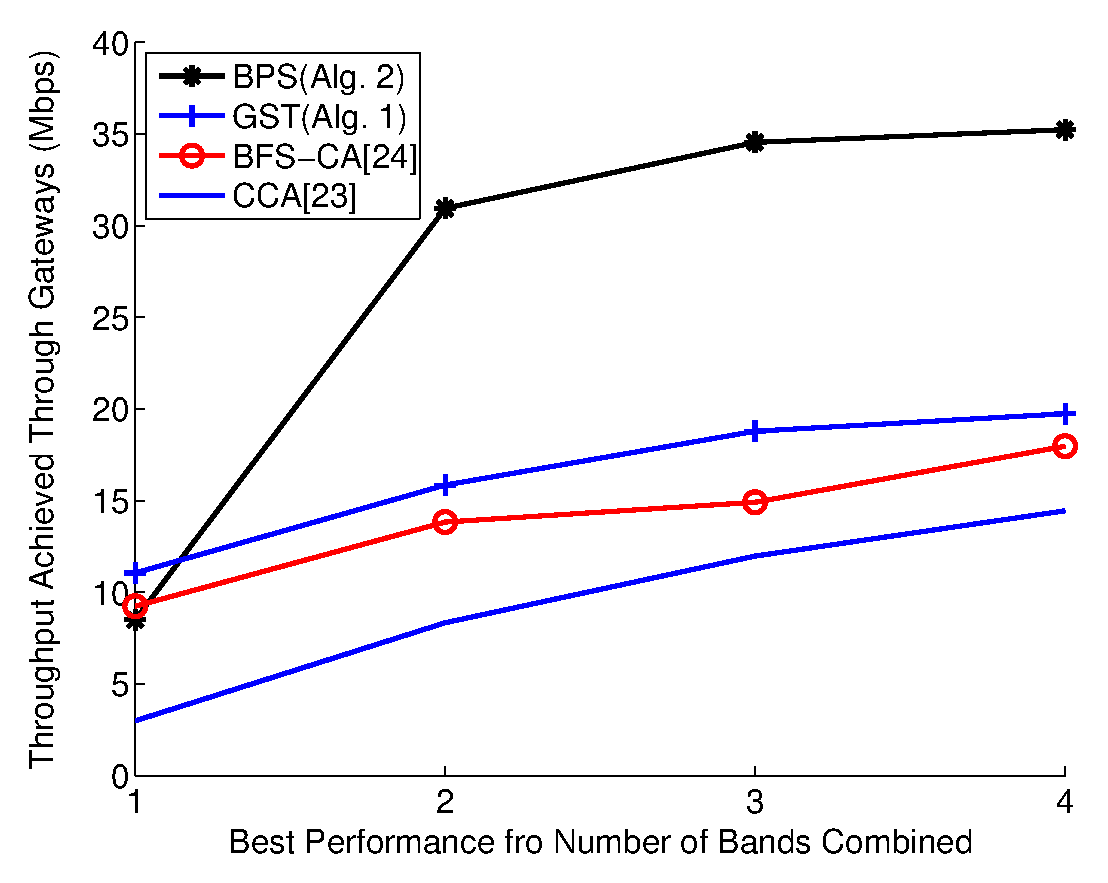
\includegraphics[width=74mm]{figures/varyradios}
\vspace{-0.1in}
\caption{Varying radios in 30-node regular-grid of 4 Mbps.}                                                                               
\label{fig:varyradios}
%\vspace{-0.0in}
\end{figure}





In ~\ref{fig:wifiws}, the performance of 4 different type of band combination is shown. 
The four curves are WiFi Only (2.4,5 GHz), WS Only (450,800 MHz), WS (450 MHz) + Multi-WiFi(2.4 GHz), Multi-WS(450, 800 MHz) + Multi-WiFi(2.4, 5 GHz). 
Increasing radios do help to improve the performance, but with the same radios and bandwidth, WiFi and white space combination could outperform only WiFi and only white space performance.

\begin{figure}
%\vspace{-0.0in}
\centering
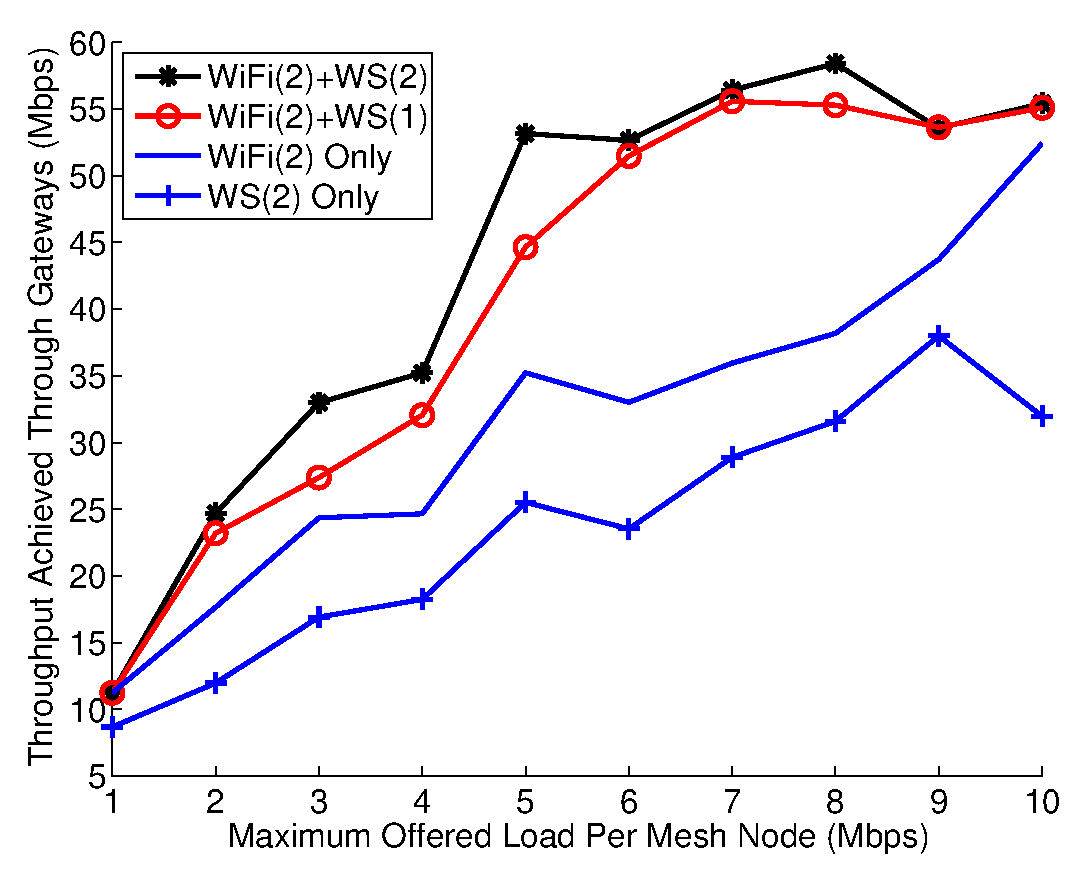
\includegraphics[width=74mm]{figures/wifiws}
\vspace{-0.1in}
\caption{BPS (Alg. 2) performance with two total channels of WiFi or white space (WS) with varying offered load from x mesh nodes.}
\label{fig:wifiws}
%\vspace{-0.0in}
\end{figure}
